% !TEX encoding = IsoLatin

\documentclass[12pt,ULlof,ULlot]{ULrapport}

% Chargement des packages supplementaires (si absent de la classe)
\usepackage[ansinew]{inputenc}
\usepackage[autolanguage]{numprint}
\usepackage{icomma}
\usepackage{hyperref}
\usepackage{placeins}
\usepackage{array}
\usepackage{amsmath}
\usepackage{longtable}
%\usepackage{amsmath}
%\usepackage[options]{nom_du_package}

% Definition d'une commande pour presenter des cellules multilignes dans un tableau
\newcommand{\cellulemultiligne}[1]{\begin{tabular}{@{}c@{}}#1\end{tabular}}

% Definition de colonnes en mode paragraphe avec alignement ajustable
% Cette definition requiert le chargement du package "array"
%    - alignement horizontal, parametre #1 : - \raggedright (aligne a gauche)
%                                            - \centering (centre)
%                                            - \raggedleft (aligne a droite)
%    - alignement vertical, parametre #2 : - p (aligne en haut)
%                                          - m (centre)
%                                          - b (aligne en bas)
%    - largeur, parametre #3 : longueur
\newcolumntype{Z}[3]{>{#1\hspace{0pt}\arraybackslash}#2{#3}}
\newcolumntype{P}[1]{>{\raggedright\arraybackslash}p{#1}}

% Definitions des parametres de la page titre
\TitreProjet{Stage �t� 2014}                         % Titre du projet
\TitreRapport{Rapport}                       % Titre du rapport
\Destinataire{D�partement de G�nie Logiciel}         % Nom(s) du destinataire
\NumeroEquipe{01}                                     % Numero de l'equipe
\NomEquipe{Aristote Diasonama}                               % Nom de l'equipe
\TableauMembres{%                                     % Tableau des membres de l'equipe
   \hline        % matricule & nom & \\\hline
   000\,000\,000  & Aristote Diasonama         & G�nie Logiciel\\\hline        % matricule & nom & \\\hline
}
\DateRemise{03 09 2014}                           % Date de remis


% Contenu de l'historique des versions
\HistoriqueVersions{%                        % version & date & description \\\hline
       &  24 aout 2013 & Cr�ation du document \\ \hline
	VF   & 03 septembre 2014 & Rapport version finale \\ \hline
%   1.3   & 14 janvier 2011 & reformatage de l'exemple, changements � l'organisation des figures\\\hline
%   1.3.1   & 24 novembre 2011 & matricules � 9 chiffres, titre du rapport\\\hline
}


% Corps du document

\begin{document}

%   Chapitres
% !TEX encoding = IsoLatin

%
% Chapitre "Introduction"
%

\chapter{Introduction}
\label{s:intro}

En �t� 2014, je faisais d�j� mon premier stage en Informatique � Wanted Technologies travaillant sur les outils internes pour la g�n�ration de rapport ainsi que quelques corrections des bugs dans l'API. � l'issu de ce stage riche en exp�rience inoubliable, j'�tais convaincu que mon choix de cursus acad�mique correspondait bien � ce que je voulais faire dans la vie.
Cet �t� je suis retourn� dans la meme entreprise, � l'occurrence Wanted Technologies mais cette fois, dans une autre �quipe, l'�quipe User Interface (UI) . C'est donc de cette experience v�cue dans l'�quipe UI qu'il sera question dans les prochaines lignes de ce rapport. 


\section{Wanted Technologies}
\label{about_wanted}

WANTED Technologies est une entreprise informatique cr�� en 1999 qui fournit de l'information de veille commerciale en temps r�el pour le march� du recrutement. La soci�t� a son si�ge social � Qu�bec, au Canada, et maintient une filiale am�ricaine ayant ses bureaux principaux � New York. Elle accumule, depuis octobre 2002, les d�tails associ�s aux offres d'emploi et maintient actuellement une base de donn�es surpassant un milliard d'offres d'emploi uniques.
Ses clients qui proviennent des secteurs tels que  les ressources humaines, les services de recrutement, les m�dias et les gouvernements utilisent WANTED Analytics, son logiciel principal,  pour identifier et prioriser les pistes de vente, cerner les tendances �conomiques, analyser les activit�s de la concurrence, estimer les conditions �conomiques futures ainsi qu'identifier des candidats pour des postes difficiles � combler.  \cite{REF01}


% !TEX encoding = IsoLatin

%
% Chapitre "Environnement de Travail"
%

\chapter{Environnement de travail}
\label{s:env_travail}
\section{Organisation de l'entreprise}
\label{sec:organisation_equipes}
Wanted poss�de des �quipes diversifi�es d'employ�s dans ses bureaux de Qu�bec. Aux cot�s des membres de la direction de l'entreprise, nous retrouvons les �quipes de marketing, d'assurance qualit�, de livraison produit, les �quipes de d�veloppeurs. Il existe une communication permanente entre ces diff�rentes �quipes ce qui permet certainement le bon fonctionnement de l'entreprise. 
Durant mon stage, je faisais �videmment partie de l'�quipe technique, l'�quipe des d�veloppeurs.
En effet, les d�veloppeurs � Qu�bec sont organis�s en 5 principales �quipes comme suit:

1. L'acquisition: Cette �quipe con�oit, entretient et maintient les logiciels qui permettent � Wanted Technologies d'obtenir les donn�es sur le march� d'emploi. Les logiciels con�us par cette �quipe, vont rechercher des donn�es sur le march� d'emploi et les mettre � la disposition des bases de donn�es de Wanted.

2. L'�quipe de base de donn�es: Cette �quipe est charg�e de la reception, l'analyse, l'organisation et la sauvegarde des donn�es que les logiciels de l'�quipe d'acquisition ram�nent � Wanted.
Les donn�es renvoy�es par l'�quipe d'acquisition sont � l'�tat pur, l'�quipe de base de donn�es va donc les traiter et les organiser de mani�re � ce qu'elles deviennent compr�hensibles et utilisables par Wanted et ses clients.

3. Le middleware: Cette �quipe est celle qui s'occupe de l'API Wanted. L'API permet aux clients de Wanted de consulter la vaste quantit� des donn�es sur le march� d'emploi qui ont �t� bien trait�es et sauvegard�es par l'�quipe de base de donn�es. L'API offre des services qui facilitent donc la consultation des donn�es par les clients.

4. L'�quipe d'interface utilisateur (UI): Cette �quipe est quant � elle charg�e de pr�senter les donn�es de Wanted via une interface web. L'�quipe UI pr�sente les donn�es de mani�re � ce qu'elles soient faciles � lire et comprendre pour les clients qui ne sont pas n�cessairement int�ress�s par les donn�es � l'�tat brut. Cette �quipe mod�lise les 
graphiques qui permettent ainsi de bien assimiler ce qui se passe dans le march� d'emploi.

5. L'�quipe d'assurance qualit� (QA): La derni�re et non la moindre, cette �quipe est charg�e d'assurer que les produits livr�s aux clients respectent bien les standards de qualit� �tablis par Wanted. Les membres de cette �quipe effectue des tests avanc�s sur les produits avant la livraison comme apr�s la livraison. Cela permet de s'assurer que les produits livr�s par Wanted sont toujours de tr�s haute qualit�.




\section{Mon Role au sein de l'�quipe}
\label{sec:about_wanted}

Sous la supervision de Gaetan Corneau, Directeur R\&D � Wanted, j'ai pass� mon stage au sein de l'�quipe middleware. 
Avec l'aide de mon chef d'�quipe, Jean-Sebastien Vachon, et tous les membres de l'�quipe, mon int�gration au sein de l'�quipe a plut�t �t� tr�s facile. J'ai eu � participer � diff�rents types de projets au sein du middleware\ref{s:taches}.
Bien que stagiaire, des t�ches de d�veloppement touchant directement � une nouvelle version majeure de Wanted Analytics m'ont �t� confi�es.





% !TEX encoding = IsoLatin

%
% Chapitre "Environnement de Travail"
%

\chapter{T�ches effectu�es}
\label{s:taches}
Durant mon stage au sein de Wanted, j'ai eu � effectuer plusieurs t�ches en relation avec ma position dans l'�quipe middleware. Dans ce chapitre, je vais d�crire trois t�ches qui ont �t� pleines de d�fis et d'opportunit�s d'apprentissage:

1. La mise en place d'un nouveau syst�me de rapport pour Wanted et ses clients \ref{sec:systeme_rapport}.
2. L'impl�mentation d'un module de s�curit� pour une application interne, la configuration centralis�e. \ref{sec:config_central}
3. L'impl�mentation des nouvelles features pour la prochaine version de Wanted Analytics \ref{sec:new_features}.

\section{Nouveau syst�me de rapport}
\label{sec:systeme_rapport}
\subsection {Le probl�me}
Wanted utilise un syst�me de rapport pour analyser l'utilisation des ses produits par ses clients. Ce syst�me permet d'obtenir les statistiques tel que le nombre de fois une application a �t� utilis�e, qui l'ont utilis�, etc..
Cependant le syst�me qui �tait en place pr�sentait beaucoup de lacunes, �tait difficile � maintenir et posait beaucoup des probl�mes � l'�quipe middleware charg�e de concevoir et maintenir ce syst�me.
C'�tait donc dans cette optique, qu'il nous a �t� charg�, avec un second stagiaire, de concevoir et mettre en place un nouveau syst�me de travail, beaucoup plus stable, facile � maintenir et surtout qui permettra une �volution rapide et la cr�ation facile de nouveaux rapports.
\subsection{La solution}
Apr�s analyse du syst�me existant et des requis pr�sent�s par les futurs utilisateurs du syst�me de rapport, nous avons envisager plusieurs possibilit�s de solution. Parmi ces solutions, nous avons eu la possibilit� de recr�er un syst�me de rapport � partir de z�ro, nous avons consid�r� r�utiliser des solutions propri�taires de syst�me de rapport comme Pentaho, Birt par Actuate , Jasper Studio par JasperSoft, Crystal etc.. et nous avons aussi consid�rer les versions libres de Birt ansi que Jasper.
Tr�s vite, nous nous sommes rendus compte que reimpl�menter le syst�me de z�ro ne serait pas une solution id�ale du point de vue ressources puisque nous aurions essentiellement reconstruit un syst�me qui faisait le m�me travail que la majorit� des solutions existantes que nous avons d�couvert. Nous avons donc proc�d� � l'analyse en profondeur des syst�mes existants. De ma part j'avais choisi d'analyser Birt, sa version tant commercial que libre. J'ai d�velopp� une petite preuve de concept de la solution que je proposais avec Birt.
Apr�s analyses et d�bats, nous avons au final choisi d'utiliser Jasper Studio et de l'adapter aux besoins de Wanted Technologies. Nous avons et reconstruits les anciens rapports  avec le nouveau syst�me et avec l'aide des autres membres de l'�quipe, nous l'avons d�ploy� pour utilisation \ref{fig:capture_jasper}.
 
\section{Module de s�curit� pour la configuration centralis�e}
\label{sec:config_central}
\subsection{Le probl�me}
La configuration centralis�e est l'application qui permet aux autres applications de Wanted d'obtenir des informations n�cessaires pour leur bon fonctionnement. � chaque fois qu'une application est lanc�e, elle interroge la configuration centralis�e pour obtenir les informations n�cessaires pour par example se connecter � la base des donn�es.
Il fallait implementer un module de s�curit� pour cette configuration centralis�e. Ce module permettra d'identifier les clients (les autres applications de Wanted) sont autoris�s � utiliser cette configuration centralis�e. L'acc�s doit donc �tre autoris� aux clients identifi�s et permis d'utiliser la configuration et il sera refus� aux autres qui n'ont pas cette autorisation.
\subsection{La solution}
Nous avons mis en place le module de s�curit� pour la configuration centralis�e. En effet, chaque client qui peut utiliser la configuration centralis�e, doit au pr�alable �tre enregistr� et avoir �t� autoris� � utiliser l'application.
On peut via une interface web enregistrer un client via son nom et son adresse. Apr�s via la m�me interface, on peut �tre en mesure d'autoriser le client enregistr� � utiliser une configuration qui aura au pr�alable �t� cr��e.
De m�me, on peut aussi annuler l'autorisation d'un client � utiliser une configuration donn�e \ref{capture_config}.


\section{Implementation des features dans la nouvelle version de WantedAnalytics}
\label{sec:new_features}

Enfin, j'ai travaill� directement sur l'api de Wanted Analytics. J'ai d�velopp� 2 nouvelles features qui feront partie de la nouvelle version internationale de Wanted Analytics qui sera disponible dans les prochains mois. 



% !TEX encoding = IsoLatin

%
% Chapitre "Environnement de Travail"
%

\chapter{Reflexion sur la formation pratique}
\label{s:formation_pratique}
Dans ce chapitre, ma formation pratique au sein de Wanted sera abord�e. Il s'agira notamment de la m�thode de d�veloppement utilis� pendant mon stage, l'organisation du travail au sein de mon �quipe du middleware et pour finir un bilan g�n�ral sur l'atteinte des objectifs fix�s pour le stage.

\section{M�thode de d�veloppement}
\label{sec:methode_developpement}
Pendant mon stage, j?ai �t� expos� � plusieurs m�thodes de travail. De mani�re generale, la methodologie de travail au sein de mon equipe etait la methodologie agile. Les taches  � effectuer �taient reparties aux �quipes selon leur domaine respectif.Ensuite au sein de l?equipe , chaque membre pouvait choisir la tache sur laquelle il voulait travailler. Le temps effectu� sur une tache est track� grace un syst�me de management des projects agiles.
Toutefois j?aimerai parler en particulier du processus des resolutions de bugs.

Pour un gros logiciel aussi utilis� que Wanted Analytics, les bugs font parties integrantes du travail journalier des developpeurs.

Les bugs sont principalement identifi�s par les clients, les analystes en qualit�, ainsi que les scripts de test de l?Application.
Une fois les bugs identif�s, ils sont transmis � l?�quipe concern�e. Ensuite un membre de l?equipe concern�e se mettra � corriger les bugs.
La correction se fait dans un premier temps dans un environnement de developpement. Une fois le bug corrig� et test� en developpement, la modification est effectu� dans un second environnement appel� staging. En staging, les analystes de qualit� vont alors tester si les bugs est vraiment resolu. Si la resolution du bug est accetp�, le travail est pass� en integration. Des tests vont s?effectuer en integration. Et la solution restera en integration jusqu?� ce qu?� la prochaine mise en production avec certainement d?autres corrections de bugs ou des nouvelles features d�j� en integration.
Au moment de la MEP, la correction va etre lanc� en production et plusieurs tests vont encore etre effectu�s pour s?assurer que la correction a bien �t� faite.
 
\section{Organisation du travail}
\label{sec:organisation_travail}
En tant que Stagiaire, les taches me furent attribu�s par le superviseur de mon �quipe. Nous commencerons par une r�union pour discuter du travail � accomplir. De la pr�sentation du probl�me � une petite analyse des possibles solutions.
Ensuite j?estime l?effort que �a me prendra d?accomplir la tache. L?effort est bas� sur l?experience personnnelle. L?effort s?exprime en nombre d?heures. La tache fait souvent partie d?un grand projet qui elle poss�de une �ch�ance. D?o� l?estimation de l?effort doit etre rationnel et reste dans le temps allou� pour le projet parent.
Dans la majorit� de cas, mes taches ont souvent prises une journ�e d?analyse profonde du probl�me qui est tr�s souvent d?une recherche des diff�rentes solutions possibles. 
Une fois ces deux �tapes pass�es, une solution est choisie et est implement�e. Des tests vont suivre pour valider la solution. Si les tests sont pass�es, le travail est termin�. Sinon on recommence avec l?analyse du probl�me et l?analyse des possibles solutions.

\section{Bilan du stage}
\label{sec:bilan_stage}

En effet l?objectif principal du stage tel que pr�sent� dans l?offre du stage �tait de concevoir et mettre en place un syst�me qui analyse les logs de services web afin de compiler des statistiques d�taill�es d'utilisation pour WANTED et ses clients.
Ce projet a pris la majeure partie de mon stage. Nous avons �t� deux stagiaires � travailler sur ce projet. 
Nous avons effectu� beacuoup d?analyse en amont, explor� beaucoup des pistes de solution avant de d�cider de la solution finale au projet. Ce projet m?a pris la moiti� du temps de stage.
Au d�part, j?�tais moins satisfait du projet � cause du temps qui �tait demand� pour l?analyse du probl�me. Cependant je me suis rendu compte de l?importance de cette �tape car cela nous a �vit� beaucoup des peines dans le future. Aujourd?hui le syst�me de rapport est en production et pour le moins que l?on puisse dire, je consid�re cette partie de stage r�ussie.
L?objectif secondaire tel que pr�sent� dans l?offre, c?�tait d?effectuer toutes taches connexes � mon poste. C?est vrai tel qu?�nonc�, cet objectif  a l?air plutot vague. Cependant, c?est dans ces taches connexes que j?ai plus trouv� du plaisir pendant mon stage.
Les t�ches que j?ai eues � faire pendant la deuxi�me partie de mon stage consistait principalement: R�soudre un bug dans Wanted Analytics, travailler sur un projet interne et ensuite travaille sur deux nouvelles features de la prochaine version de Wanted Analytics. Toutes ces taches ayant bien �t� effectu�es et compl�t�es, je consid�re cette partie de stage compl�tement r�ussie.

En effet l?objectif principal du stage tel que pr�sent� dans l?offre du stage �tait de concevoir et mettre en place un syst�me qui analyse les logs de services web afin de compiler des statistiques d�taill�es d'utilisation pour WANTED et ses clients.
Ce projet a pris la majeure partie de mon stage. Nous avons �t� deux stagiaires � travailler sur ce projet. 
Nous avons effectu� beacuoup d?analyse en amont, explor� beaucoup des pistes de solution avant de d�cider de la solution finale au projet. Ce projet m?a pris la moiti� du temps de stage.
Au d�part, j?�tais moins satisfait du projet � cause du temps qui �tait demand� pour l?analyse du probl�me. Cependant je me suis rendu compte de l?importance de cette �tape car cela nous a �vit� beaucoup des peines dans le future. Aujourd?hui le syst�me de rapport est en production et pour le moins que l?on puisse dire, je consid�re cette partie de stage r�ussie.
L?objectif secondaire tel que pr�sent� dans l?offre, c?�tait d?effectuer toutes taches connexes � mon poste. C?est vrai tel qu?�nonc�, cet objectif  a l?air plutot vague. Cependant, c?est dans ces taches connexes que j?ai plus trouv� du plaisir pendant mon stage.
Les t�ches que j?ai eues � faire pendant la deuxi�me partie de mon stage consistait principalement: R�soudre un bug dans Wanted Analytics, travailler sur un projet interne et ensuite travaille sur deux nouvelles features de la prochaine version de Wanted Analytics. Toutes ces taches ayant bien �t� effectu�es et compl�t�es, je consid�re cette partie de stage compl�tement r�ussie.



\section{Commentaires sur la recherche de stage, formation pr�-stage et Orientation de carri�re}
\label{sec:commentaires}

De la formation pr�-stage, je crois que deux cours ont �t� vraiment tr�s important pour le contenu de mon stage, le cours de g�nie logiciel orient� object (GLO-2004), ainsi que le cours du processus en genie logiciel. Le cours de GLO-2004 a mis les bases pour le langage Java que j?ai utilis� pendant mon stage. Aussi l?analyse que nous avons effectu�e pendant le projet de session pour ce cours m?a servi de base pour l?analyse que j?ai eue � effectuer au d�but de stage. D?autre part, le cours de processus en genie logiciel a �t� aussi d?une importance capitale surtout que c?est le cours qui m?a introduit au processus de d�veloppement en entreprise et sp�cialement au processus en g�nie logiciel. Ce qui a permis que je me sente d�j� � l?aise avec la terminologie et les concepts de base du processus que j?ai utilis� durant mon stage.
Avec ces deux connaissances acquises et une experience en tant que d�veloppeur dans un projet � l?universit� Laval, j?�tais sur que j?avais ce qu?il fallait pour me trouver un stage. La recherche de stage a �t� plutot facile pour moi. D�s que j?ai vu l?offre de Wanted, c?etait ce que j?ai cherch�. Tout s?est pass� correctement et j?ai eu mon stage rapidement.
Avec ce stage r�ussi, je n?ai jamais �t� aussi convaincu que c?est bien dans le g�nie logiciel que je veux faire carri�re. Cependant j?ai encore du mal � choisir dans quelle concentration je vais me lancer, je voudrais faire du logiciel industriel mais je pense que j?appr�cie enormement le d�veloppement web et mobile. Pour l?instant, pendant que je me donne encore le temps � reflechir sur ma concentration future, j?ai choisi de continuer � travailler dans tous les domaines o� l?on r�soud les probl�ms rencontr�s chaque jour.

%!TEX encoding = IsoLatin

%
% Chapitre "Reflexion th�orique"
%

\chapter{Reflexion sur la formation th�orique}
\label{s:reflexion_theorique}
La formation th�orique re�ue � l?universit� a �t� en majeure partie tr�s utile dans mon stage. S?il y a une recommandation que je devrais faire au directeur de programme, c?est d?essayer de trouver des voies et moyens pour encourager des activit�s pratiques au sein du programme d?informatique et du g�nie logiciel pendant lesquelles les �tudiants pourront appliquer toutes les th�ories r��ues en classe. La th�orie est bonne mais n?est pas suffisante pour am�liorer la capacit� de r�action face aux nouveaux probl�mes qui se posent. Il faudra encourgaer les activit�s pratiques de programmation tel que les hackatons.
En parlant de formation th�orique, j?aimerai un eclaircissement sur le concept d?architecture logicielle emergente de la part de mon professeur d?introduction au processus en genie logiciel.
Avant mon stage je voulais suivre un cours optionnel en d�veloppement web. Toutefois j?ai appris beaucoup sur le web pendant mon stage que je crois que je vais suivre un cours optionnel en d�veloppement mobile.




%!TEX encoding = IsoLatin

%
% Chapitre "Introduction"
%

\chapter{Conclusion}
\label{s:conclusion}
Apr�s mon interview, j?�tais convaincu que mon stage serait une exp�rience enrichissante. Mon superviseur de stage, Mr Gaetan avait r�ussi en m?en persuader. A la fin du stage, je ne peux qu?affirmer que mon intuition �tait bien correcte!
En effet, avant mon stage, j?avais suivi le cours d?Introduction au processus g�nie logiciel. De ce cours, j?avais appris diff�rentes �tapes principales du developpement logiciel comme la phase de r�quis, d?analyse, d?implementation, d?integration, de tests, etc..
Cependant pendant mon stage, au d�but, j?avais clairement sous estim� l?importance de la phase d?analyse dans le d�veloppement logiciel.
Toutefois, grace � l?�quipe enti�re, j?ai su d�couvrir l?importance de cette phase analytique au fil du temps et je m?y suis donn� � coeur joie.
Tous ces concepts je les avais bien maitris�s, pendant mon stage je les ai mis en pratique, je sais l?importance de l?analyse dans une conception logicielle et je sais comment le faire pratiquemet.
Mon developpement en java, en a aussi beaucoup profit�. Et le plus evidemment, c?est l?efficacit� que j?ai maintenant avec l?outil Eclipse. J?ai appris beaucoup des raccourcis et beaucoup de hacks qui ont augment� ma productivit� avec Eclipse.
 

% !TEX encoding = IsoLatin
\chapter{Annexe}

\begin{figure}[!ht]
\centering
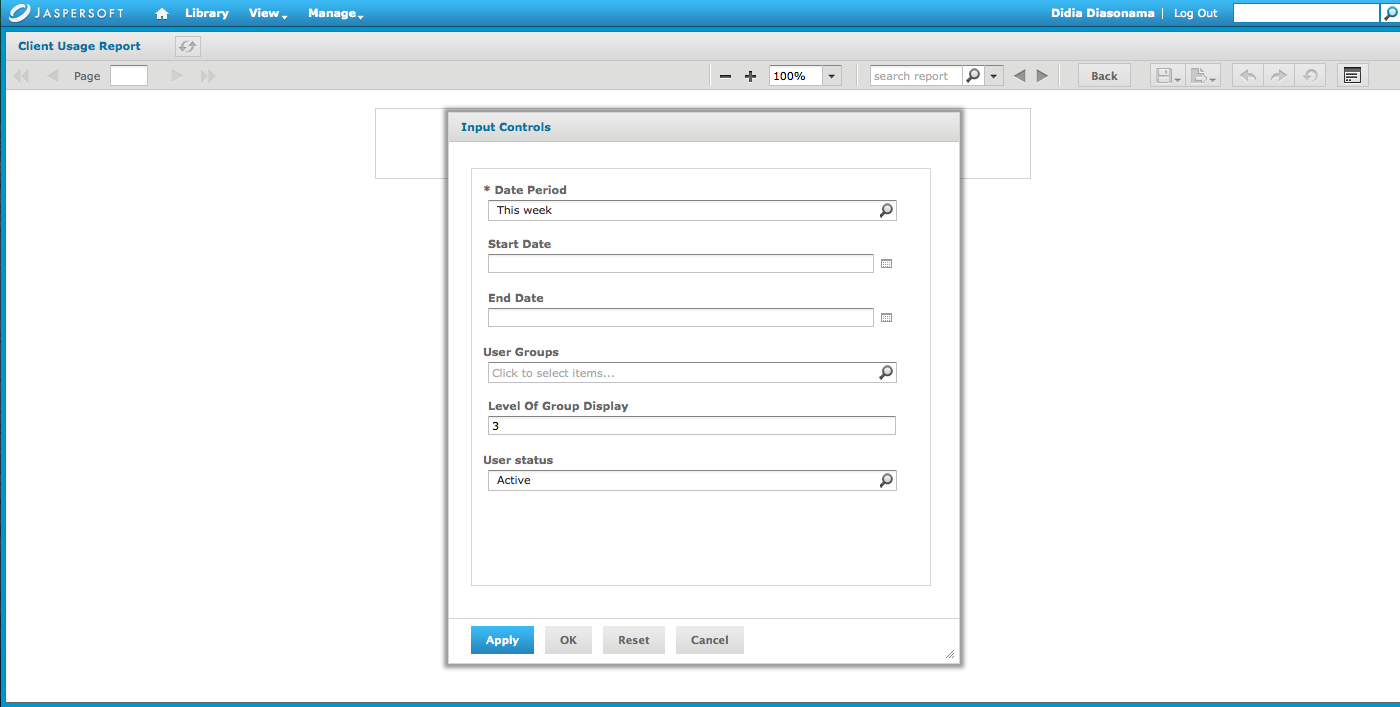
\includegraphics[scale=1, width = 16cm, height = 12cm ]{fig/jasper.png}
\caption{Capture d'�cran Jasper Report Server}
\label{fig:capture_jasper}
\end{figure}
\begin{figure}[!ht]
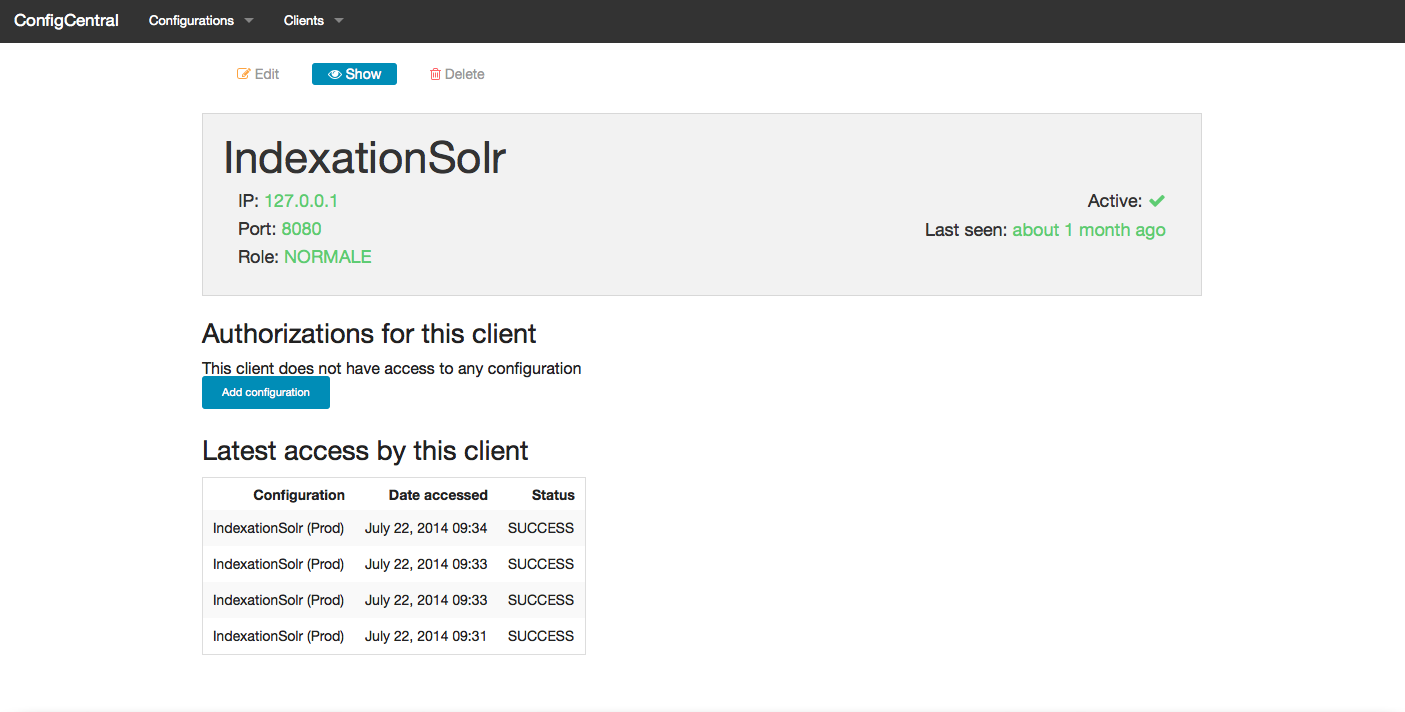
\includegraphics[scale=1, width = 16cm, height = 12cm ]{fig/config_central.png}
\caption{Capture d'�cran Configuration centrale}
\label{fig:capture_config}
\end{figure}
\begin{figure}[!ht]
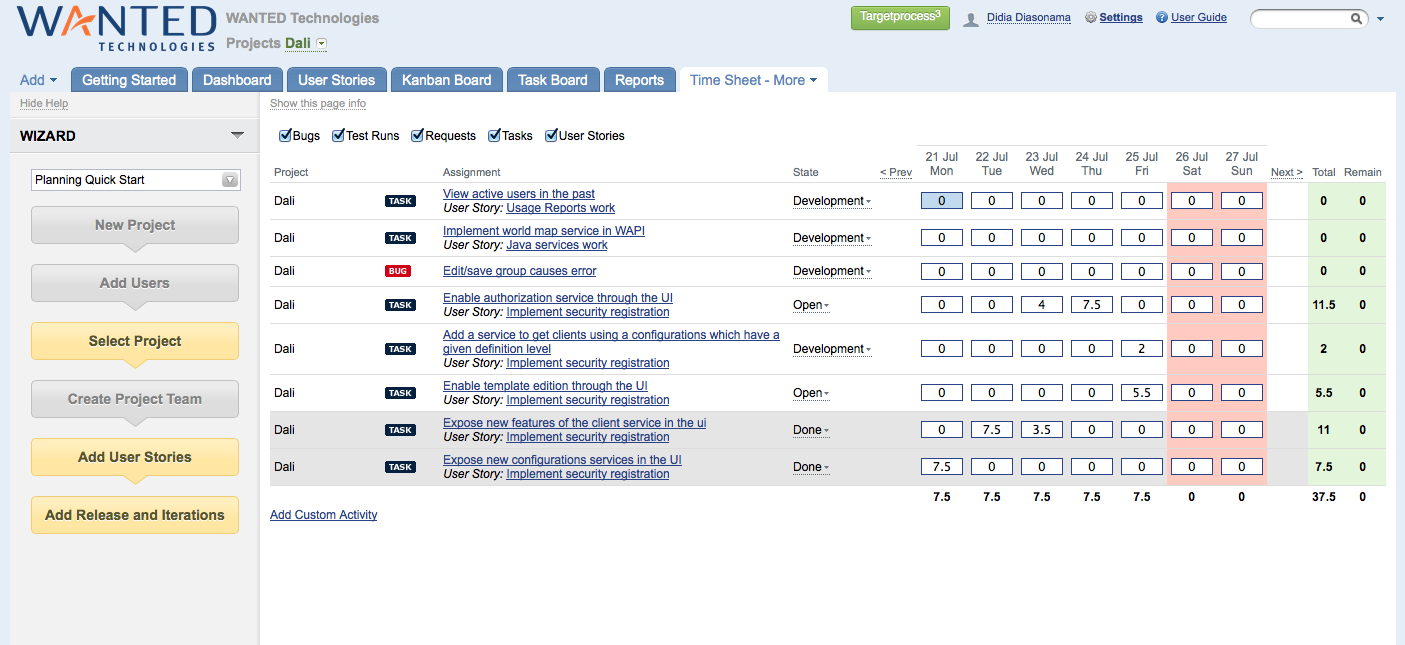
\includegraphics[scale=1, width = 20cm, height = 12cm ]{fig/timesheet.png}
\caption{Capture d'�cran timesheet}
\label{fig:capture_timesheet}
\end{figure}
\clearpage


%!TEX encoding = IsoLatin

%
% Chapitre "Bibliographie"
%

\begin{thebibliographyUL}{99} % remplacer le "{9}" par "{99}" lorsque le nombre de references
                              % requiert 2 caracteres (>= 10 references)

\bibitem{REF01} Wanted Technologies. \emph{A propos de nous}, [En ligne]. \url{https://www.wantedanalytics.com/fr/a-propos/a-propos-de-nous} (Page consult�e le 24 aout 2014)
 \end{thebibliographyUL}







%   Annexes
%\appendix
%\input{tex/liste_sig_acr}

\end{document}
% Fin du document

